
\documentclass{article}

\usepackage{tcolorbox}
\usepackage{minted}
\usepackage{geometry}
\geometry{
  a4paper,
  total={210mm,297mm},
  left=25mm,
  right=25mm,
  top=30mm,
  bottom=30mm,
}

\begin{document}
\title{Vagrant Puppetmaster demo}
\author{Marc Lambrichs}

\maketitle

\begin{abstract}
First goal is to create a test environment for any application or set of applications using a central - but local! - vagrant box running puppetmaster, r10k and puppetdb.

In a different project we're creating a test environment with a combination of Elasticsearch, Logstash, Kibana (ELK-stack), combined with redis for caching. Having your own test environment allows you to develop and test your own puppetmodules, before pushing them on into a CI pipeline.
\end{abstract}

\section{Prerequisites}
Your environment should contain:
\begin{enumerate}
\item git
\item ruby
\item vagrant
\item virtualbox
\item and finally, some rubygems:
\begin{enumerate}
\item vagrant-cachier
\item vagrant-hosts
\item vagrant-vbguest
\end{enumerate}
\end{enumerate}
Example: installing vagrant-cachier:

\begin{minted}[bgcolor=black,formatcom=\color{white},fontsize=\footnotesize]{bash}
marc:~ marc$ sudo gem install vagrant-cachier
\end{minted}

\section{Structure}
The puppetmaster functionality is split up in 3 separate repositories.
\begin{enumerate}
\item puppetmaster
\item hiera
\item r10k
\end{enumerate}

\par All three of them, are - separate - git repositories, with different purposes. The \emph{puppetmaster} repo contains a Vagrantfile that serves as our starting point for building a puppetmaster. The other two repositories, \emph{r10k} and \emph{hiera} are being used during the puppetmaster install to create a complete production-like environment of puppetmaster on a vagrant box. Our first goal is to install puppetmaster, so we can leave the \emph{hiera} and \emph{r10k} repo's, for now.

\par So check out the puppetmaster repository in a directory of your liking.

\begin{minted}[bgcolor=black,formatcom=\color{white},fontsize=\footnotesize]{bash}
marc:~ marc$ mkdir vagrant
marc:~ marc$ cd vagrant
marc:~ marc$ git clone git@cassandra.melange-it.nl:/var/opt/git/generic/puppetmaster.git puppetmaster
marc:~ marc$ cd puppetmaster
marc:~ marc$ git submodule update --init --recursive
\end{minted}

\par Before building, you need to add your own entry in puppetmaster/config/boxes.yaml.

\par Now, you're ready to install your own puppetmaster.

\section{Boxes}

To start up a puppetmaster using vagrant, we need to have a basic vagrant box upon which we put our necessary software. The definition of boxes you need are defined in the file config/boxes.yaml.
Obviously, you could use your own box or get one from a public repo.\\
Take a look at https://atlas.hashicorp.com/boxes/search or http://vagrantbox.es.

\section{Step 1: Puppetmaster}

\subsection{Puppetmaster, r10k, puppetdb and foreman in one go}
Cd into your puppetmaster directory and start up vagrant.

\begin{minted}[bgcolor=black,formatcom=\color{white},fontsize=\footnotesize]{bash}
marc:~ marc$ cd ~/vagrant/puppetmaster
marc:puppetmaster marc$ vagrant up
\end{minted}

This will start off a lot of output, ending with a \emph{puppet apply} on your vagrant box. Next thing to do, is to check if everything is working.

\subsection{Check and doublecheck}

\par First, let's check if your puppetdb is running. Open your browser with http://puppet.arthurjames.vagrant:8080 and you should see something like this:\\
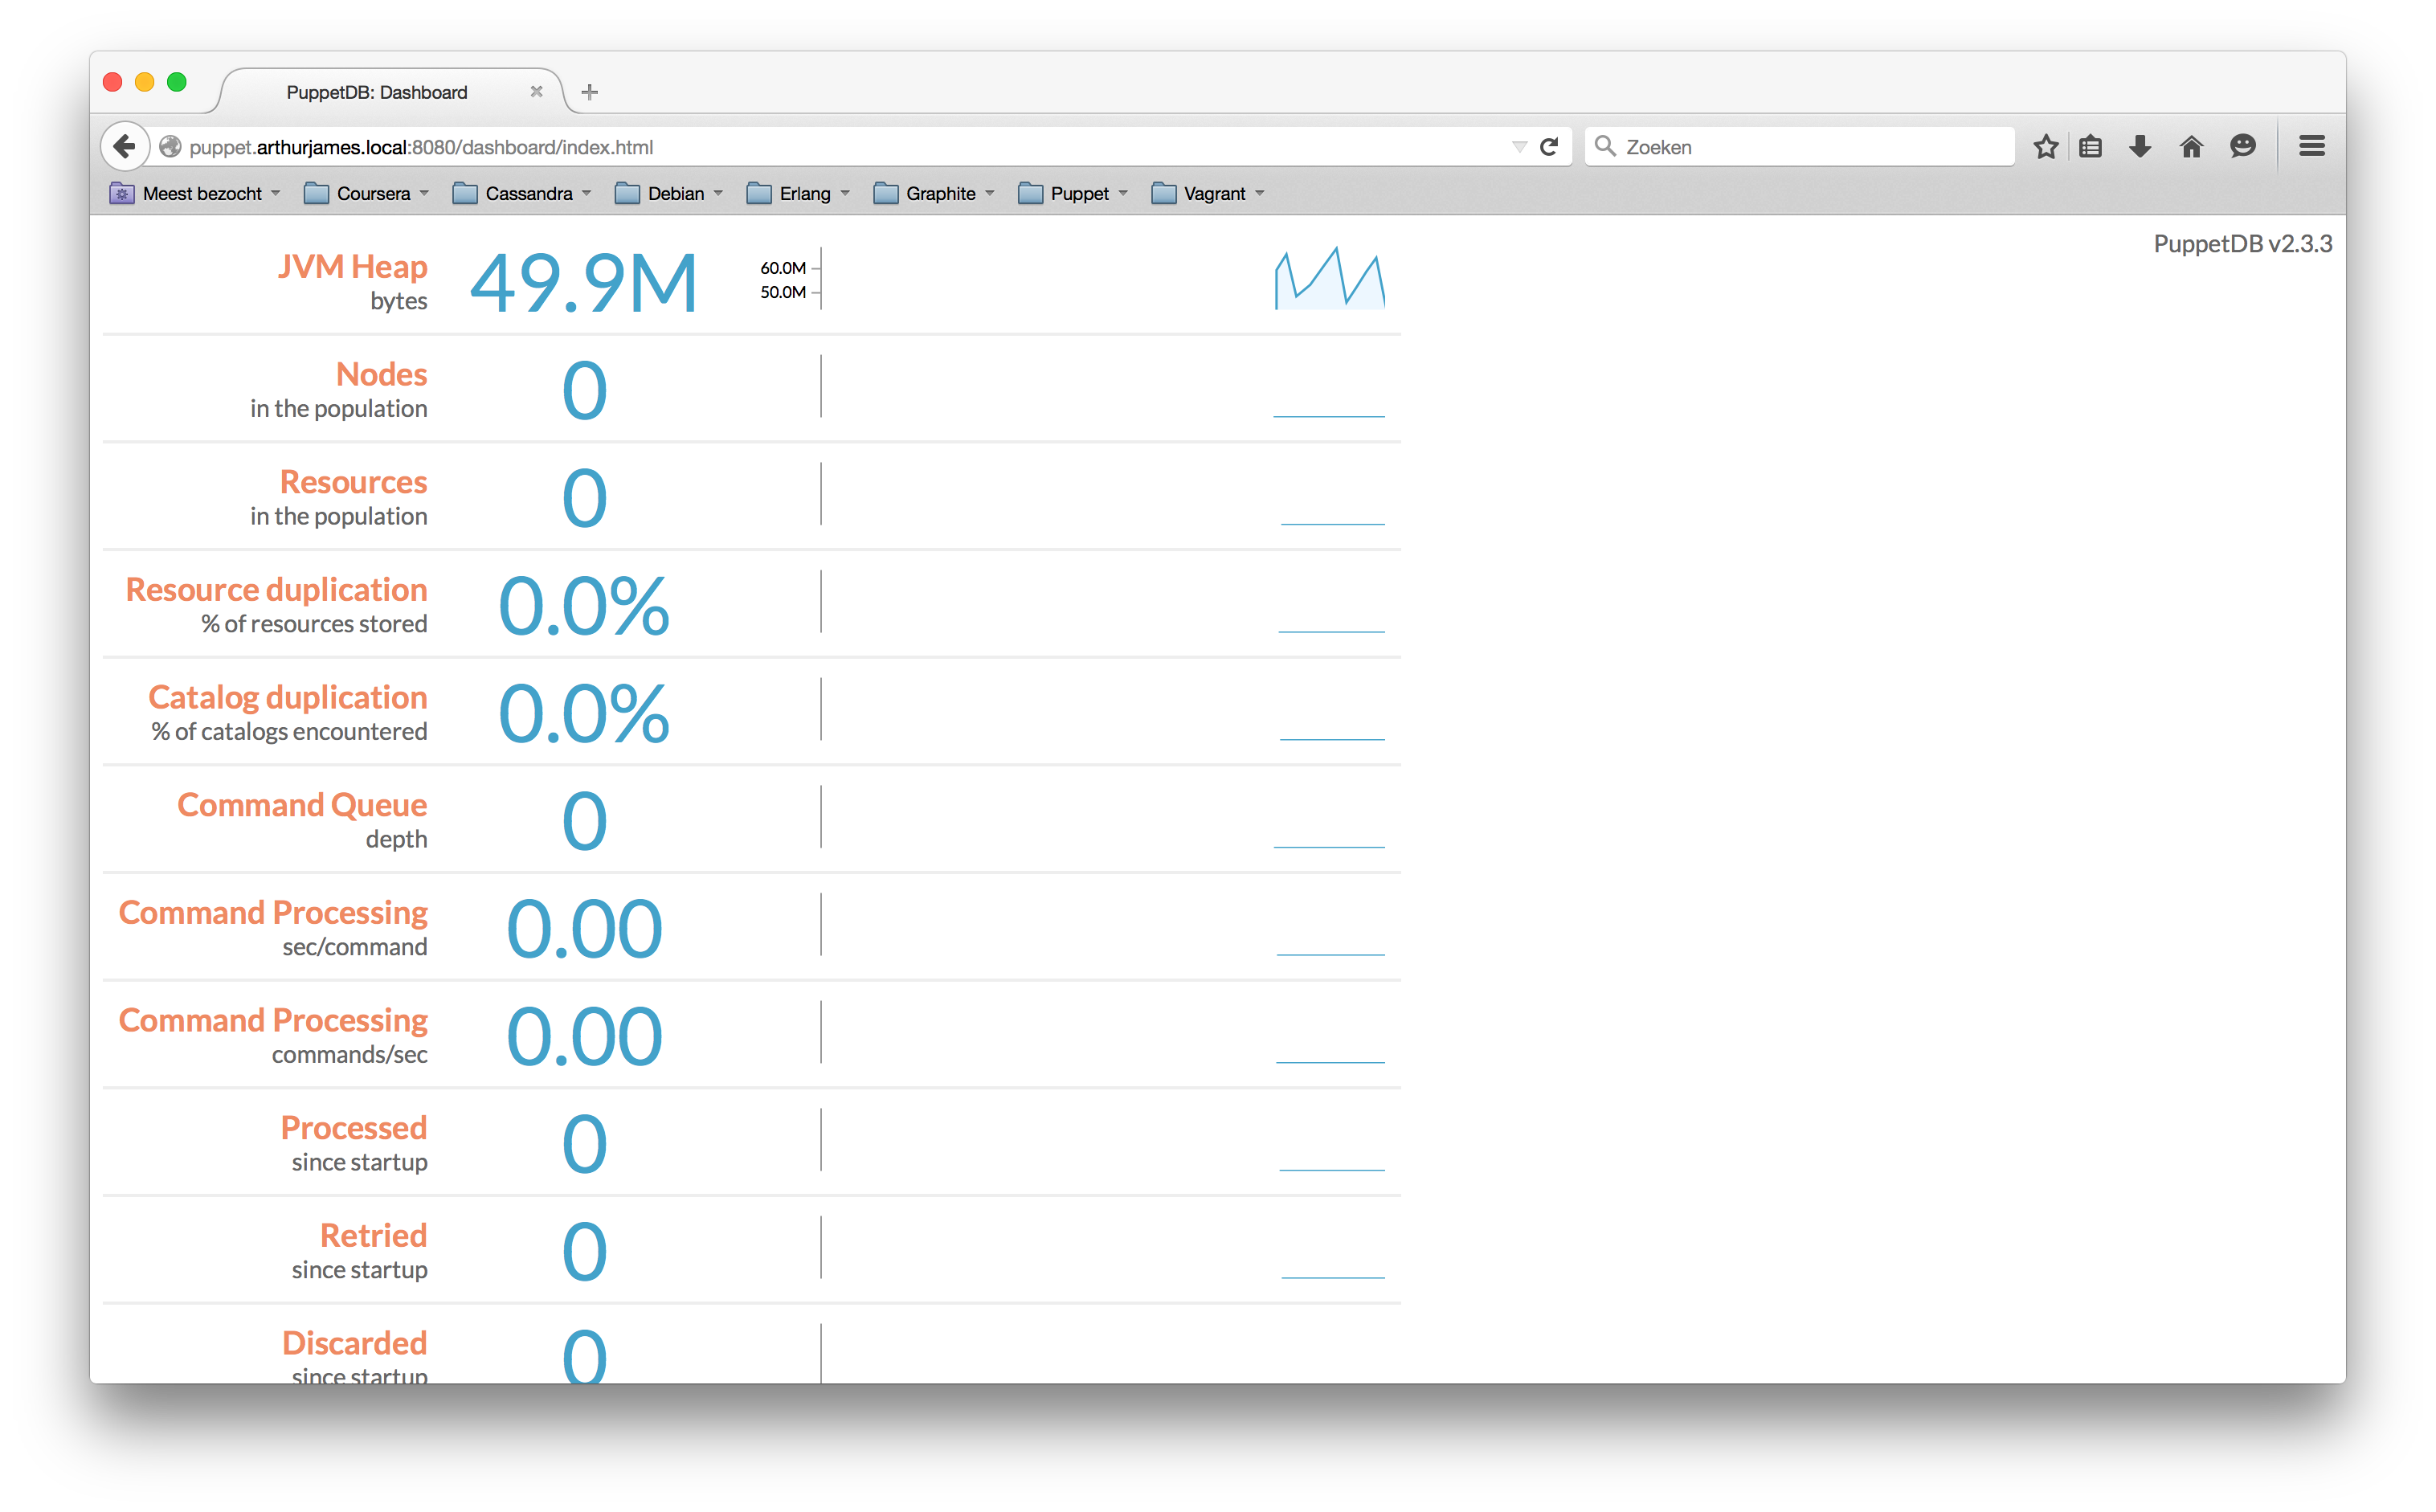
\includegraphics[scale=0.3]{images/puppetdb}


\par Next, check if you can access foreman. On the same host on port 80 you should see:\\
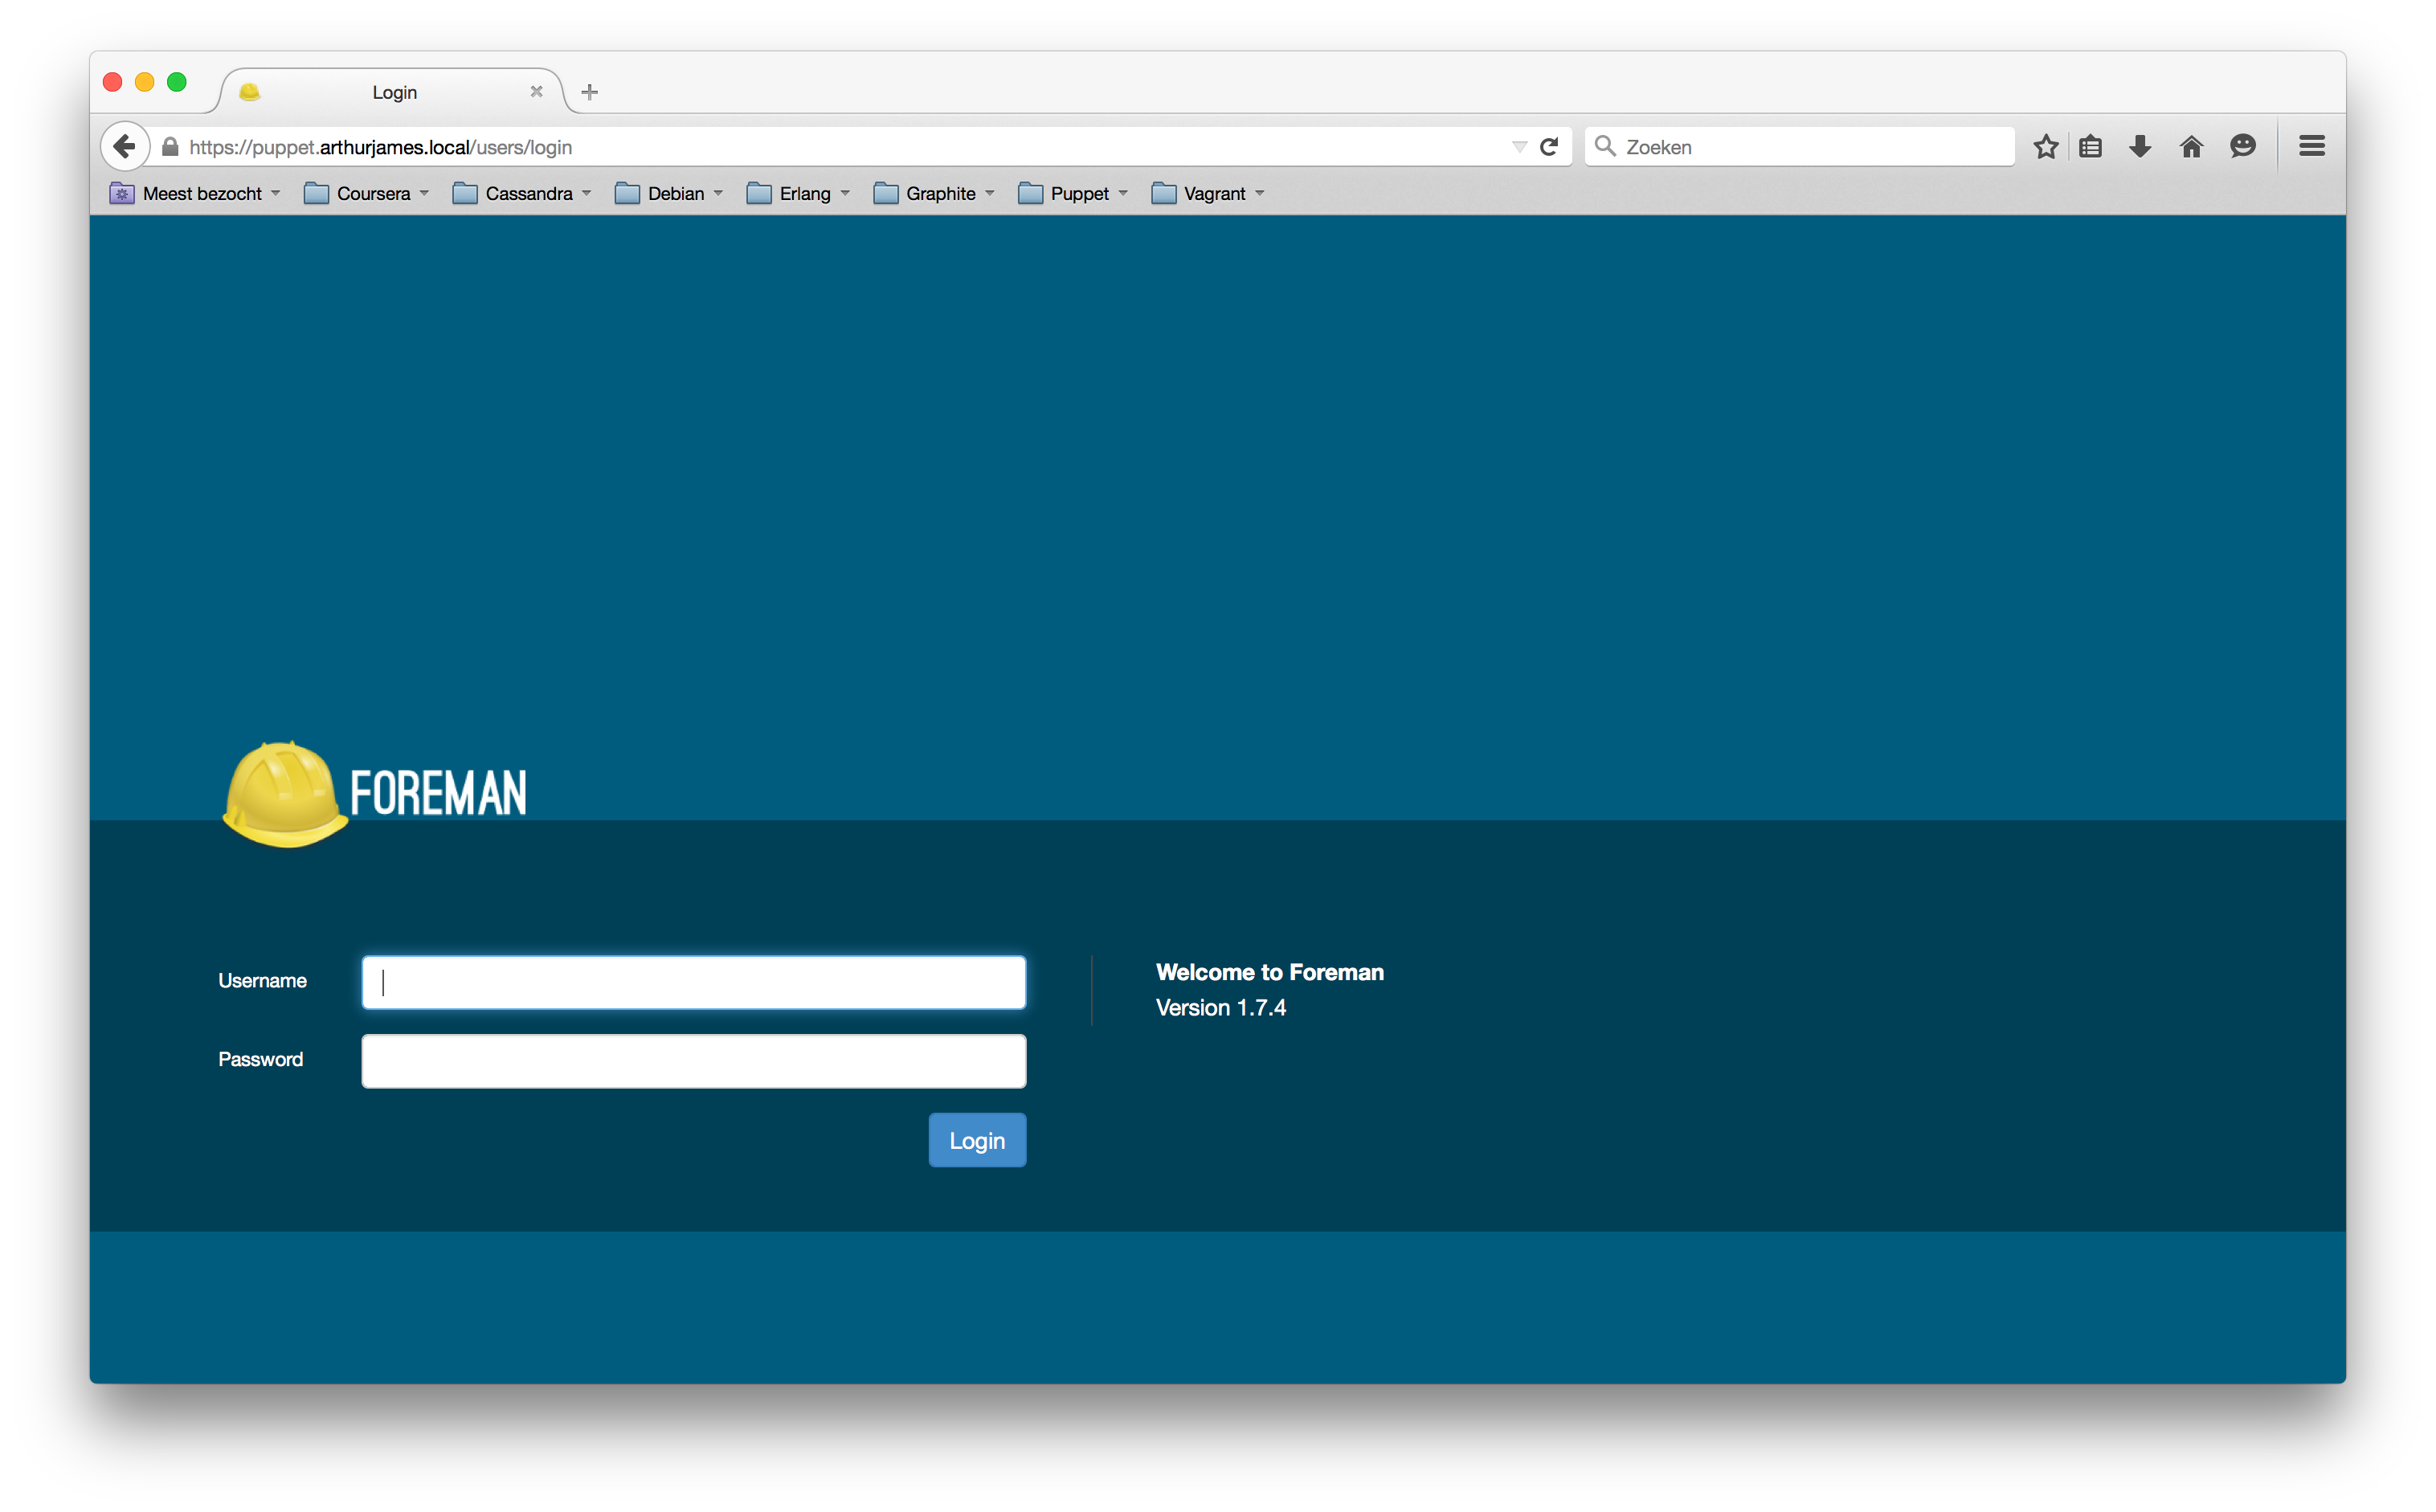
\includegraphics[scale=0.3]{images/foreman}

\par If you can, check if you can log in to foreman with credentials \emph{admin/changeme}.
\par Probably no nodes have been recognized, so there are two options here:
\begin{itemize}
\item wait for 30 min (the default setting inbetween puppet agent runs)
\item ssh into your vagrant box to kick off a puppetrun.
\end{itemize} 

\begin{minted}[bgcolor=black,formatcom=\color{white},fontsize=\footnotesize]{bash}
marc:~ marc$ cd ~/vagrant/puppetmaster
marc:puppetmaster marc$ vagrant ssh
Linux debian 3.2.0-4-amd64 #1 SMP Debian 3.2.65-1+deb7u1 x86_64

The programs included with the Debian GNU/Linux system are free software;
the exact distribution terms for each program are described in the
individual files in /usr/share/doc/*/copyright.

Debian GNU/Linux comes with ABSOLUTELY NO WARRANTY, to the extent
permitted by applicable law.
Last login: Tue Apr 28 12:47:02 2015 from 10.0.2.2
vagrant@puppet:~$
\end{minted}

\par Now you're logged in, do:\\
\begin{minted}[bgcolor=black,formatcom=\color{white},fontsize=\footnotesize]{bash}
vagrant@puppet:~$ sudo puppet agent -v -t
\end{minted}

After the puppetrun, you should be able to see 1 node defined.\\
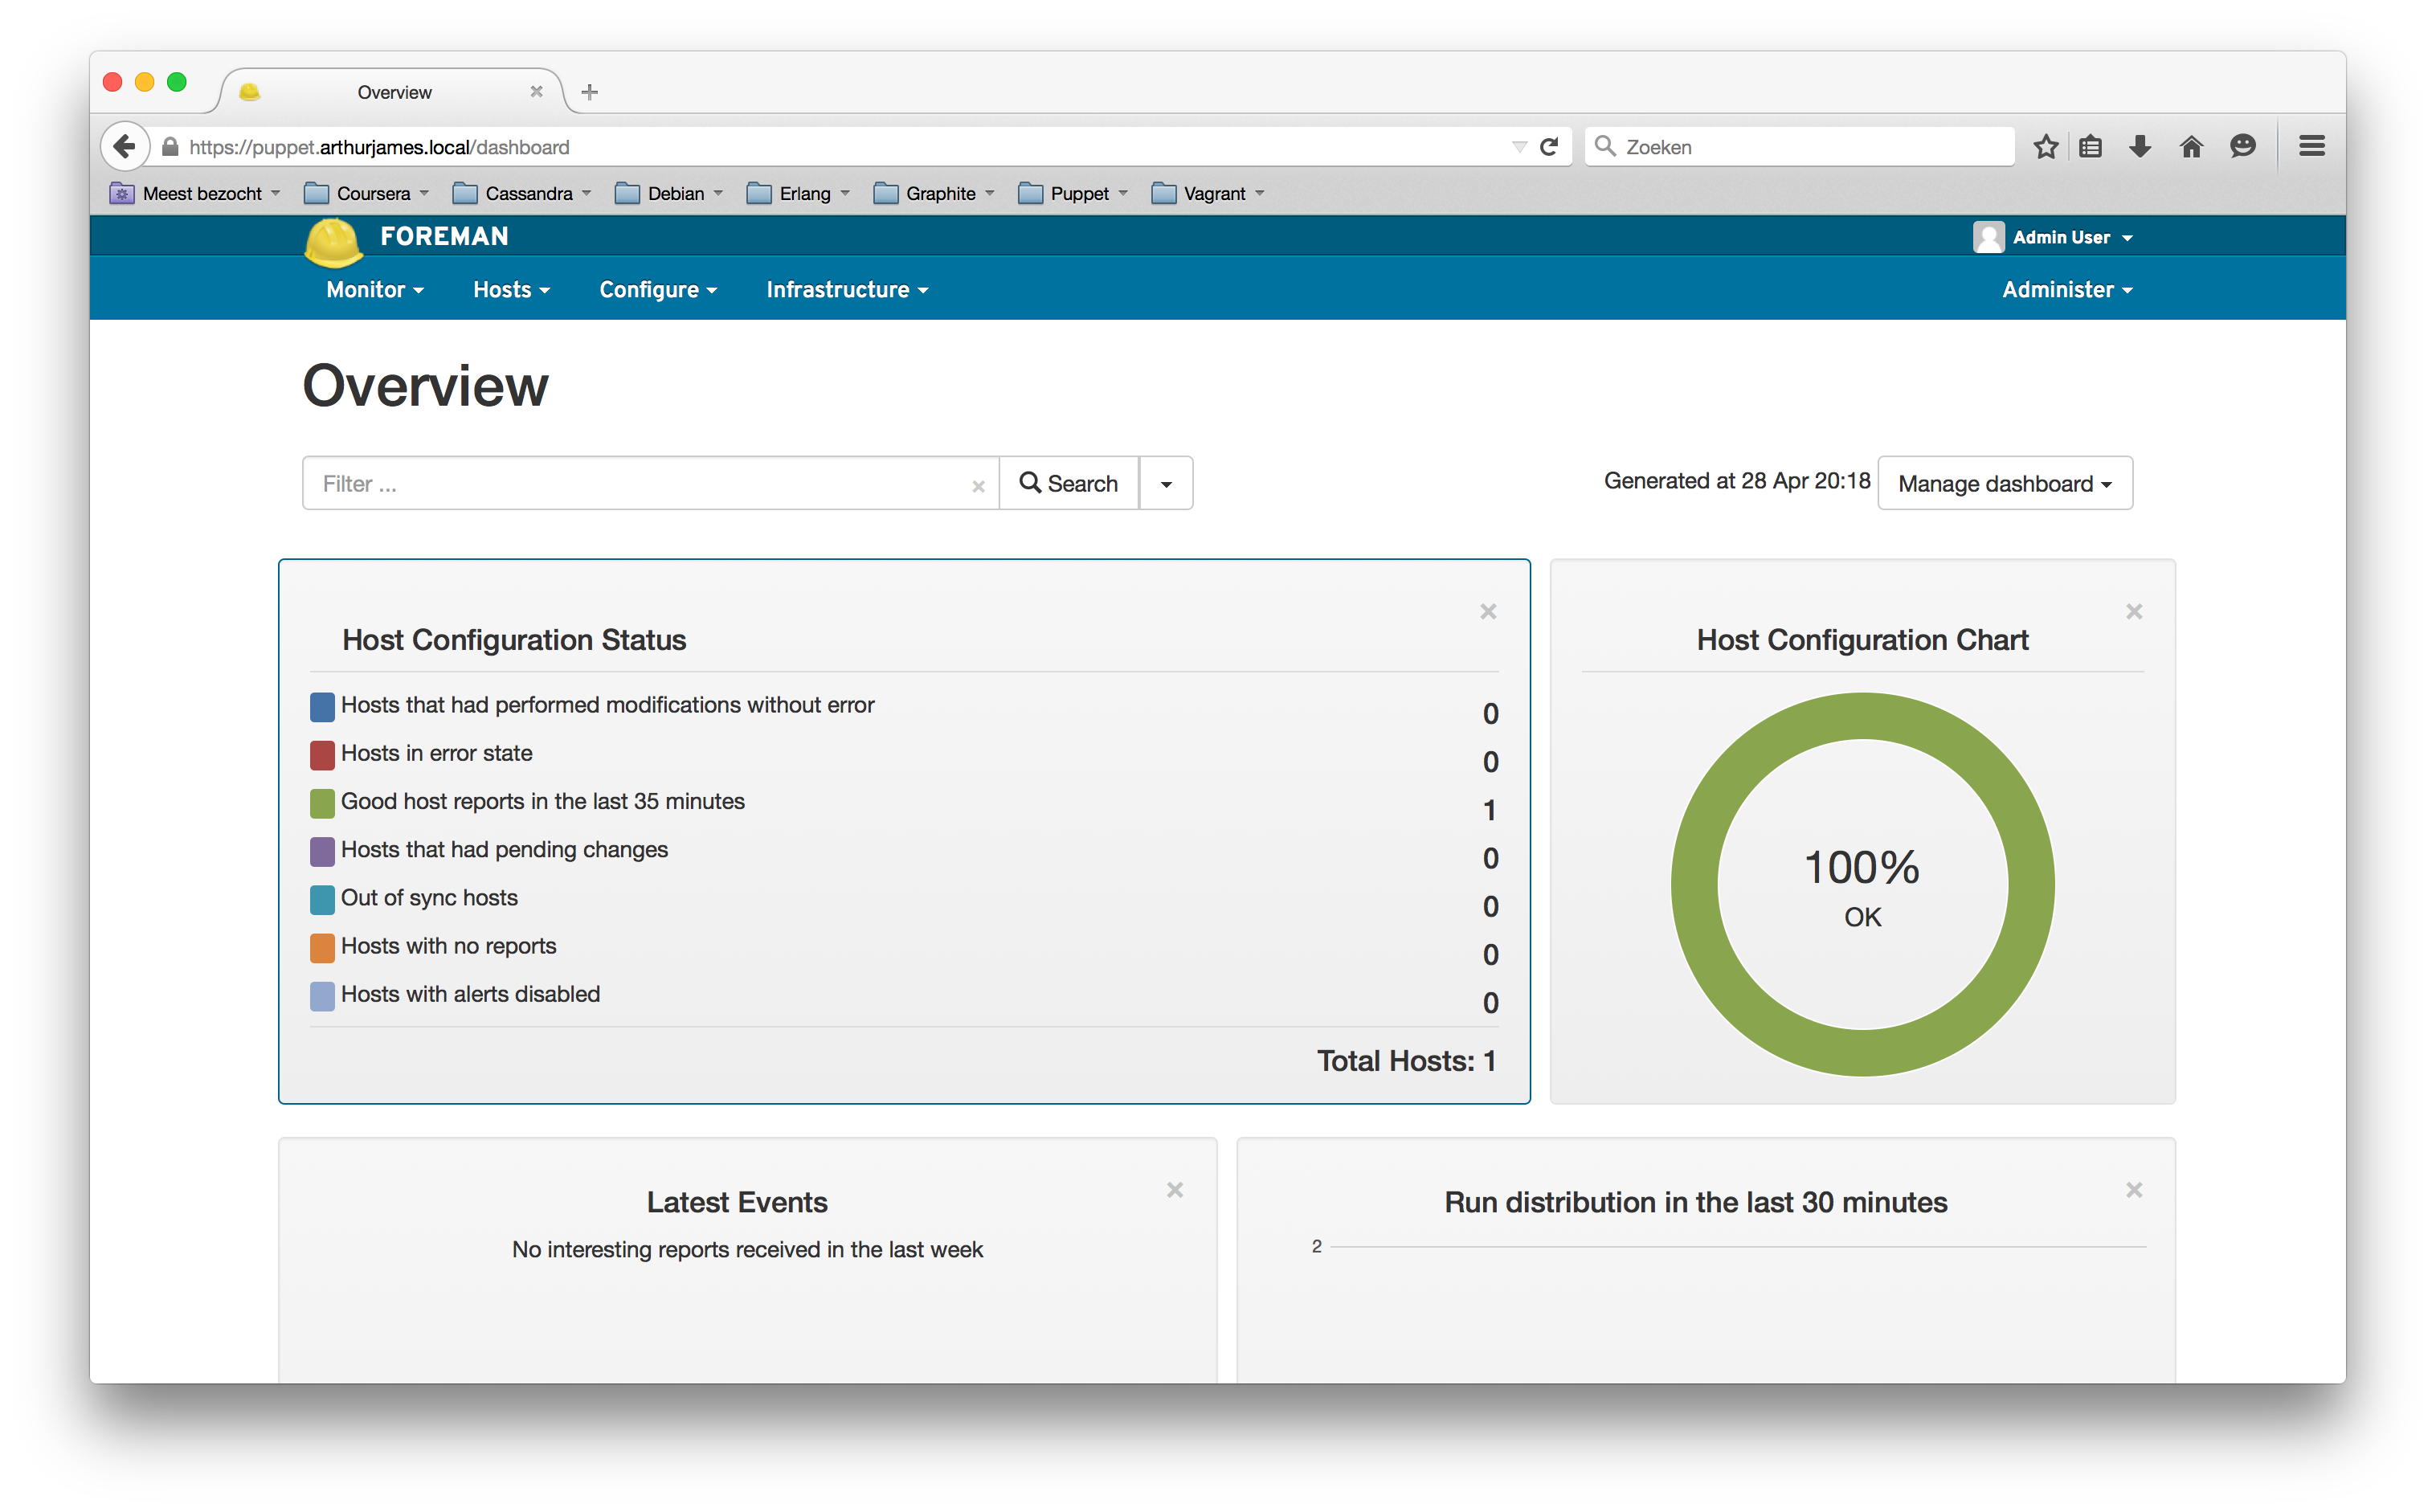
\includegraphics[scale=0.3]{images/dashboard}

\section{Step 2: Elasticsearch box}
\subsection{native box}




\section{Clients}
\subsection{Elasticsearch}
\subsection{Kibana}
\subsubsection{Kibana 3}

\subsubsection{Kibana 4}

\subsection{Logstash}

\subsection{Redis}

\end{document}
